%/*
% * SPDX-FileCopyrightText: 2021 Stefan Begerad <stefan@begerad.de>
% *
% * SPDX-License-Identifier: GPL-3.0-or-later
% */

\begin{frame}
  \frametitle{Datenaufkommen über Mobilfunk}
  Dede Bordrechner und Dede Server tauschen Daten per Mobilfunk aus.
  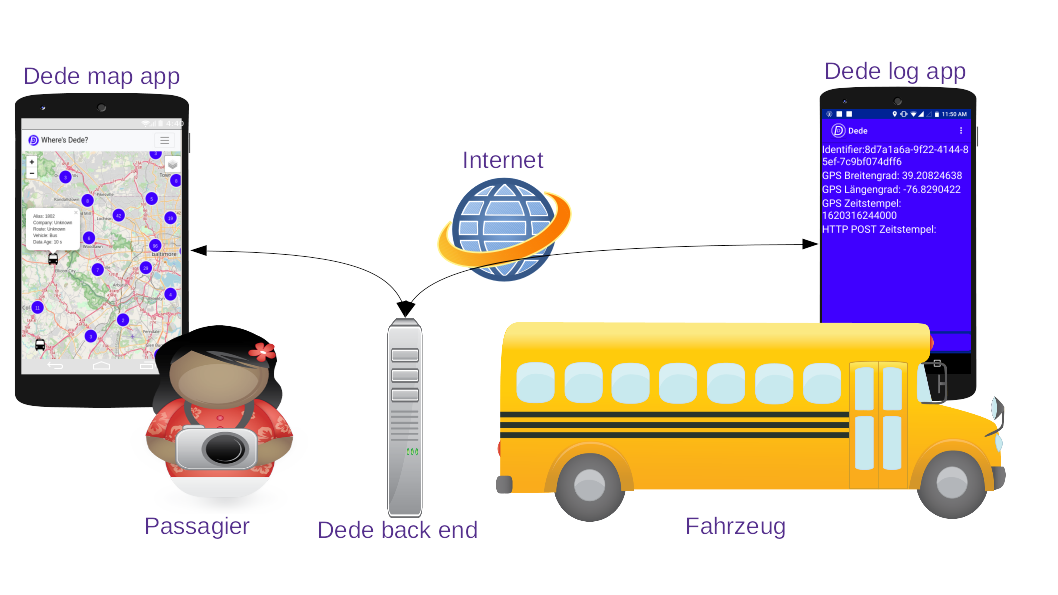
\includegraphics[width=\paperwidth]{dede/dede-concept}
\end{frame}

\begin{frame}
  \frametitle{Datenaufkommen über Mobilfunk}
  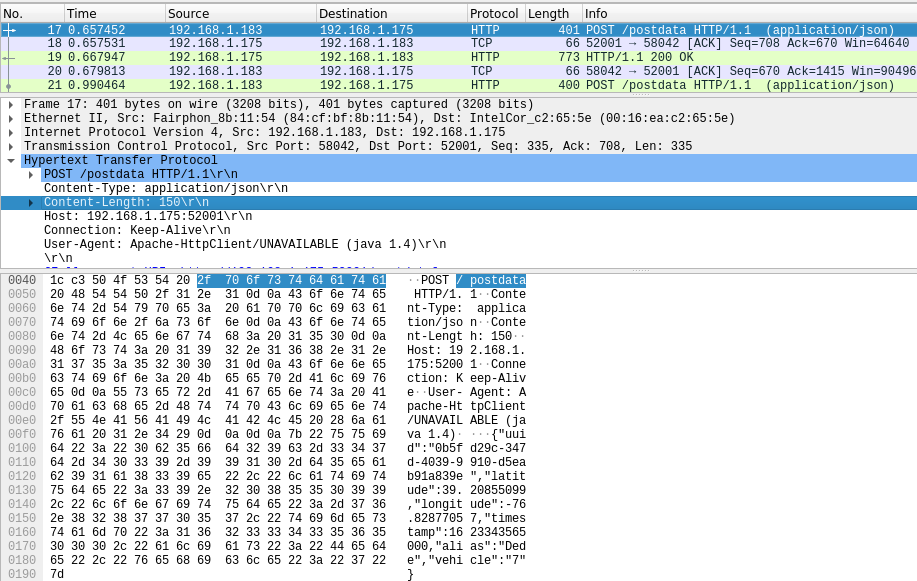
\includegraphics[width=0.88\paperwidth]{dede/dede-obc-wireshark-http-post}
\end{frame}

\begin{frame}
  \frametitle{Datenaufkommen über Mobilfunk}
  \begin{itemize}
  \item Pro Positionserfassung erstellt der Dede Bordrechner ein Datenobjekt in einer Größe von 150 Byte.
  \item Der Dede Bordrechner sendet eine HTTP POST-Anfrage in einer Größe von 401 Byte.
  \item Es resultiert ein Datenaufkommen von 1239 Byte pro Positionserfassung.
  \end{itemize}
  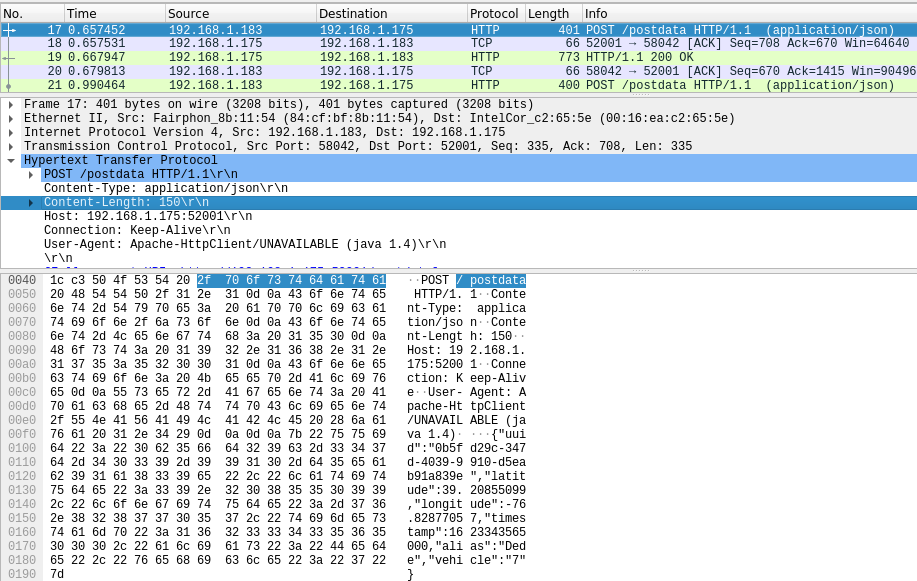
\includegraphics[width=0.5\paperwidth]{dede/dede-obc-wireshark-http-post}
\end{frame}

\begin{frame}
  \frametitle{Datenaufkommen über Mobilfunk}
  Annahme: Der Dede Bordrechner erfasst die Position einmal pro Minute.
  \begin{itemize}
  \item Datenaufkommen pro Minute: 1239 Byte/ 1,24 KByte
  \item Datenaufkommen pro Stunde: 74,34 KByte
  \item Datenaufkommen pro Tag: 1,78 MByte
  \item Datenaufkommen pro Monat: 55,31 MByte
  \item Datenaufkommen pro Jahr: 651,22 MByte
  \end{itemize}
  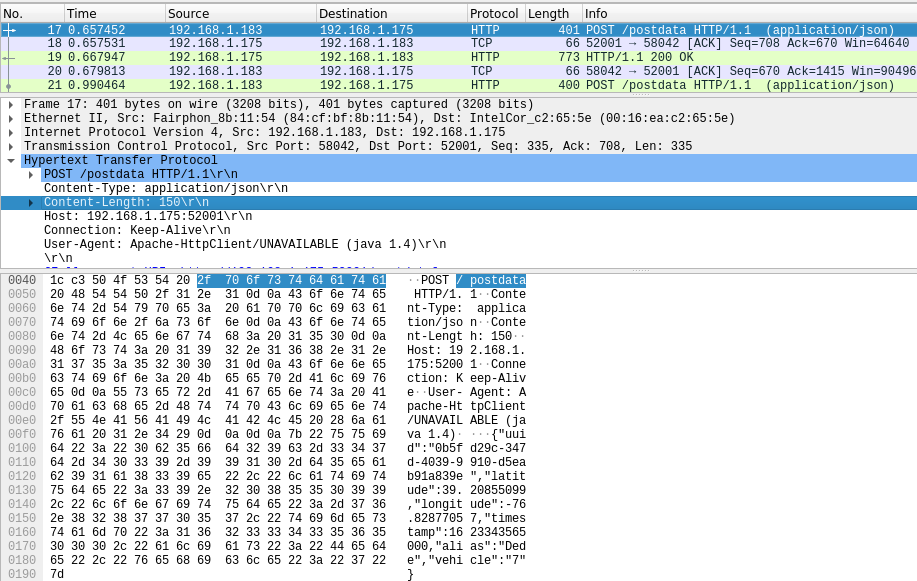
\includegraphics[width=0.5\paperwidth]{dede/dede-obc-wireshark-http-post}
\end{frame}
